\section{Experiments} \label{sec:exps}

We employ \textbf{one unified GWM model across multiple tasks}, comparing its performance against domain-specific methods. Initially, we introduce the tasks within the GWM framework.

\xhdr{Task description} 
The details of the tasks are summarized across three aspects in Table \ref{tab:dataset_all} of the Appendix, with further information on tasks and datasets available in Appendix \ref{app:dataset}, and specific action node prompts in Appendix \ref{sec:prompt}.

\begin{itemize}[leftmargin=1em, itemsep=0pt]

\item \textbf{World prediction}: It contains three subtasks. \textbf{(1) Multi-modal generation and matching (Multi-modal):} We investigate the node-level multi-modal generation task, where the goal is to predict missing images based on textual captions. We use data from Goodreads \citep{jin2024instructg2i} and the Multi-Modal-Paper dataset (detailed in Appendix~\ref{ap:multi-modal generation and matching g}). The generated images are evaluated using CLIP Score \citep{radford2021learning} and DINOv2 \citep{oquab2023dinov2}. We compare our approach against several baselines, including Stable Diffusion 1.5 (SD-1.5) \citep{rombach2022high}, its fine-tuned variant (SD-1.5 FT), the image-to-image model ControlNet \citep{zhang2023adding}, and the SOTA INSTRUCTG2I model \citep{jin2024instructg2i}. Meanwhile, our edge-level multi-modal matching task evaluates the correspondence between different modalities, using Contrastive MLP \citep{liu2022mlp}, CLIP \citep{radford2021learning}, and fine-tuned CLIP on metrics such as Accuracy, Recall, and F1. %Goodreads serves as a literature graph with nodes representing books' titles and images linked by similar-book semantics, while Multi-Modal-Paper, sourced from arXiv, comprises nodes with images, tables, and text, including captions, structured around paper references. 
Please note that since the multi-modal matching task of Multi-Modal-Paper also includes matching between text and tables, CLIP cannot be applied to this subtask.   

\textbf{(2) Recommendation (Rec):} As Table~\ref{tab:rec_data} of Appendix \ref{apd:rec} illustrates, we utilize three benchmark datasets of varying scales—Baby, Sports, and Clothing—from Amazon's real-world product collections \citep{mcauley2015image}. These datasets are commonly used in existing multi-modal graph recommendation systems \citep{mmgcn, grcn}. For these edge-level tasks, we benchmark our GWM model against recent state-of-the-art recommendation approaches, including FREEDOM \citep{zhou2023tale}, as well as representative graph-based models such as LightGCN \citep{he2020lightgcn}, MMGCN \citep{wei2019mmgcn}, and GRCN \citep{wei2020graph}. We use Recall and F1 Score as the primary evaluation metrics.  \textbf{(3) Traditional graph prediction (Graph):}  We utilize Cora \citep{chen2024exploring}, PubMed \citep{chen2024exploring}, and HIV \citep{wu2018moleculenet} datasets. For the Cora and PubMed datasets, we perform node-level and edge-level tasks, while for the HIV dataset, we undertake graph-level tasks. We compare GWM  against two traditional graph baselines, GCN \citep{kipf2016semi} and GAT \citep{velivckovic2017graph}, as well as two GFM baselines, LLAGA \citep{chen2024llaga} and OFA \citep{liu2023one}. We adopt accuracy as the metric. Details can be seen in Appendix \ref{apd:graph}.

\begin{table}[!tbp]
\setlength\tabcolsep{3pt}
\centering
\begin{footnotesize}
\vspace{-4mm}
\caption{\textbf{Multi-modal generation results on Goodreads and Multi-Modal-Paper}. This task is to predict the missing modality based on the given modality. Compared to specific baselines in image generation, GWM achieved the best results.} %
\label{tab:multi-modal generation}
\resizebox{0.43\textwidth}{!}{
\begin{tabular}{ccccc}
\toprule
& \multicolumn{2}{c}{\texttt{Goodreads}} & \multicolumn{2}{c}{\texttt{Multi-Modal-Paper}}  \\ \cmidrule(lr){2-3} \cmidrule(lr){4-5}
\textbf{Model} & CLIP   & DINOv2   & CLIP   & DINOv2    \\ \midrule
SD-1.5 & 42.16 &14.84  & 52.62 & 23.64\\
SD-1.5 FT  &\underline{45.81} &18.97  & 58.49  & 24.13 \\ 
ControlNet  &42.20  &19.77  & 52.89 & \underline{24.77}\\ \midrule
INSTRUCTG2I & \textbf{50.37} & \textbf{25.54} & 56.37 & 18.80 \\ \midrule
GWM-T &  47.46 & 20.91 & \textbf{59.92} & 23.10 \\
GWM-E & 45.23 & \underline{20.87} & \underline{59.84}  & \textbf{26.03}  \\
\bottomrule
\end{tabular}
}
\end{footnotesize}
\end{table}

\begin{table}[!tbp]
\setlength\tabcolsep{3pt}
\centering
\begin{footnotesize}
% \vspace{-1mm}
\caption{\textbf{Multi-modal matching results on Goodreads and Multi-Modal-Paper}. It aims to predict the correspondence between different modal-ities. For Goodreads, this task is to predict text-image correspondences. As for Multi-Modal-Paper, it aims to predict text-image, text-table, and table-image correspondences. Note that CLIP and CLIP FT cannot be applied to Multi-Modal-Paper since it includes matching tasks beyond text-image.} %
\label{tab:Multi-modal matching}
\resizebox{0.49\textwidth}{!}{
\begin{tabular}{ccccccc}
\toprule
 & \multicolumn{3}{c}{\texttt{Goodreads}} & \multicolumn{3}{c}{\texttt{Multi-Modal-Paper}}  \\ \cmidrule(lr){2-4} \cmidrule(lr){5-7}
\textbf{Model} & Accuracy  & Recall  & F1 Score & Accuracy  & Recall  & F1 Score \\ \midrule
Contrastive MLP &  54.70 & 54.67 & 54.79& 51.77 & 51.55 & 50.31\\ \midrule
CLIP & 83.80 & 83.80 & 83.84 & - & -& - \\
CLIP FT   & \textbf{92.60} & \textbf{92.58} & \textbf{92.61} & -& - & -   \\ \midrule
GWM-T   &84.22  &85.66  &85.29  & 88.26   &90.35   &90.11  \\
GWM-E &\underline{88.82}  &\underline{89.73}  &\underline{89.06}  & \textbf{96.23}   & \textbf{97.21}  & \textbf{97.13}   \\
\bottomrule
\end{tabular}
}
\end{footnotesize}
% \vspace{-4mm}
\end{table}

\item \textbf{World generation}: It contains two sub-tasks. \textbf{(1) Multi-agent collaboration (Multi-agent):} We utilize a multi-modal agent benchmark called AgentClinic \citep{schmidgall2024agentclinic} (in Appendix \ref{apd:agent}) to evaluate LLMs within simulated clinical environments. This environment is structured as a graph, with nodes representing different profile-based agents such as patients, measurements, and moderators, and containing various modalities of external knowledge including medical images and patient records. The edges represent interactions between agents and their engagement with knowledge resources. Given the objective of integrating information from all agents to answer medical questions, we define this as a graph-level task. We compare our approach with three LLM-based baselines: CoT \citep{wei2022chain}, ToT \citep{yao2024tree}, and Few-Shot \citep{madotto2021few}, as well as two additional baselines fine-tuned on the AgentClinic dataset. FT refers to a LLaMA-3-8B model fine-tuned directly on the task. Longformer \citep{beltagy2020longformer} is a strong baseline for long-document understanding. We use Accuracy, Recall, and F1 Score as evaluation metrics to assess the correctness of the generated responses.  \textbf{(2) Retrieval-augmented generation (RAG):} We utilize LongBench v2 \citep{bai2024longbench}, a benchmark designed for challenging long-context question-answering (in Appendix \ref{apd:RAG}). %This benchmark consists of 503 challenging multiple-choice questions, with contexts ranging from 8k to 2M words, across six major task categories. The questions are categorized into easy and hard levels, determined by the difficulty experienced by human experts and models in answering them. 
Following previous work like GraphRAG \citep{edge2024local}, we divide long context into chunks as nodes of the graph, and the edges between nodes are the similarity of their BERT embeddings. We conduct comparisons with two RAG-based baselines—BM25 \citep{robertson2009probabilistic} and Dragon \citep{lin2023train}—and three long-context LLMs ($128k$), including Mistral Large 2, Command R+, and GPT-4o mini. Accuracy serves as our evaluation metric.

\item \textbf{World optimization (Optimization)}:  Many existing works \citep{ho2016generative,hussein2017imitation,yang2024embodied} attempt optimization tasks by imitating the trajectory of expert strategies. Here, we utilize the expert strategy dataset from the text-based embodied task ALFWorld \citep{shridhar2020alfworld,yang2024embodied}. %It includes descriptions of the expert's strategy state at each decision step (comprising both images and text) as well as the decisions made (text). The action node of GWM is to prompt GWM to predict the next expert decision. to assess the ability to imitate expert strategies 
We model each decision state as graph nodes and derive the edges between nodes based on the similarity of the state images associated with the decisions.  We compare GWM with three LLM baselines—COT \citep{wei2022chain}, TOT \citep{yao2024tree}, and T5 \citep{raffel2020exploring} fine-tuned on our dataset (T5 FT) —using BERT-Score \citep{zhang2019bertscore} (Precision, Recall, and F1 Score) as metrics. Details can be seen in Appendix \ref{apd:opt}. 



\end{itemize}


\begin{table}[!tbp]
\setlength\tabcolsep{3pt}
\centering
\begin{footnotesize}
\vspace{-1mm}
\caption{\textbf{Recommendation on Baby, Sports, and Clothing}. Compared with three classical graph baselines, GWM achieved state-of-the-art results on most metrics.} %
\label{tab:Recommender systems}
\resizebox{0.48\textwidth}{!}{
\begin{tabular}{cccccccccc}
\toprule
& \multicolumn{2}{c}{\texttt{Baby}} & \multicolumn{2}{c}{\texttt{Sports}} & \multicolumn{2}{c}{\texttt{Clothing}} \\ \cmidrule(lr){2-3} \cmidrule(lr){4-5} \cmidrule(lr){6-7}
\textbf{Model}   & Recall  & F1 Score   & Recall  & F1 Score & Recall  & F1 Score \\ \midrule
FREEDOM & 60.35 & 66.16 & 63.47 & 70.53 & 70.20 & \underline{78.40} \\
\midrule
LightGCN & 51.11 & 38.22 & \underline{85.36} & \textbf{91.32} & 69.08 & 77.21 \\
MMGCN & 57.34 & 61.31 & 61.69 & 68.08 & 64.09 & 71.26 \\
GRCN & \underline{74.35} & \underline{82.47} & 57.31 & 61.23 & 57.60 & 61.74 \\ \midrule
GWM-T &  70.84 & 75.08  & 84.29 & 88.60   & \underline{71.73} & 74.26    \\
GWM-E  & \textbf{76.72} & \textbf{84.74}  & \textbf{88.78} & \underline{90.32}   & \textbf{75.27} & \textbf{84.06}  \\
\bottomrule
\end{tabular}
}
\end{footnotesize}
\end{table}


\begin{table}[!tbp]
\setlength\tabcolsep{5pt} % 设置列间距
\centering
\begin{footnotesize}
% \vspace{-1mm}
\caption{\textbf{Traditional graph prediction results on Cora, PubMed, and HIV}. It covers representative tasks at the node-level, edge-level, and graph-level. Compared to classic graph baselines and GFM methods, our GWM can match their performance with one unified model.}%It covers representative tasks at the node-level, edge-level, and graph-level. Compared to classic graph baselines and GFM methods, our GWM can match their performance with one unified model. 
\label{tab:Traditional graph prediction}
\resizebox{0.4\textwidth}{!}{
\begin{tabular}{lccccccc}
\toprule
\textbf{Model} & \multicolumn{2}{c}{\texttt{Cora}} & \multicolumn{2}{c}{\texttt{PubMed}} & \multicolumn{1}{c}{\texttt{HIV}} \\ \cmidrule(lr){2-3} \cmidrule(lr){4-5} \cmidrule(lr){6-6}
Task Type & Node   & Link  & Node   & Link  & Graph  \\\midrule

GCN & 78.86  & 90.40  &74.49  &91.10  &86.72  \\
GAT & 82.76  & \underline{93.70}  &75.24  &91.20  &87.84   \\ \midrule
LLAGA &\textbf{89.22}   & 89.18   &\textbf{95.03}   &89.18   & 85.42  \\ 
OFA &73.21  & 93.12  &77.80  &\textbf{96.39}  &92.04  \\ \midrule
GWM-T &81.92  &88.24  &\underline{92.91}  &91.88  &\underline{92.20}  \\
GWM-E &\underline{83.03}  & \textbf{94.31}  & 84.22  &\underline{94.01}  &\textbf{93.86}  \\
\bottomrule
\end{tabular}
}
\end{footnotesize}
% \vspace{-6mm}
\end{table}  %% GWM-G 




\xhdr{Implementation details} We train and test \textit{a single GWM} on all tasks, comparing it with domain-specific baselines for each task. Specifically, for the LLM module, we uniformly use Llama-3-8B, and for stable diffusion, we use SD-v1-5. For the image-to-text model used in GWM-T, we use LLaVA-1.5-7B. The image encoder and text decoder used in GWM-E are CLIP and BERT models, respectively. In addition, our multi-hop projector uses an n-hop MLP to aggregate features from different hops, where n-hop refers to the number of neighborhood hops of the graph nodes used. To ensure the training efficiency of the models, we set the maximum token length for all models at 2k. We use Adam optimizer \citep{diederik2014adam} for model training and gradually decay the learning rate with LambdaLR scheduler. All the experiments are conducted on NVIDIA A6000 GPUs. Please refer to Appendix \ref{sec:hyper} for other implementation details.


\begin{table}[ht]
\setlength\tabcolsep{3pt}
\centering
\begin{footnotesize}
% \vspace{-6mm}
\caption{\textbf{Multi-agent collaboration results on AgentClinic}. This task is to answer medical questions by leveraging interactions between agents and external knowledge sources. Compared to classic LLM baselines, GWM-T achieves state-of-the-art results.} %This task is to answer medical questions by leveraging interactions between agents and external knowledge sources. Compared to classic LLM baselines, GWM-T achieves state-of-the-art results.
\label{tab:Multi-agent collaboration}
\resizebox{0.35\textwidth}{!}{
\begin{tabular}{cccc}
\toprule
\textbf{Model} & Accuracy  & Recall  & F1 Score \\ \midrule
COT & \underline{45.00} & 33.42 & 32.25 \\
TOT &  35.00  & 33.71 & 29.71 \\ 
Few-shots & 40.00 & 40.63 & 29.37 \\\midrule
Longformer & 25.00 & 20.20 & 14.00 \\ 
FT & \underline{45.00} & \underline{45.40} & \underline{44.00} \\ 
\midrule
GWM-T & \textbf{50.00}   &\textbf{46.42}  &\textbf{48.20}  \\
GWM-E &\underline{45.00}  &39.57  & 35.56  \\
\bottomrule
\end{tabular}
}
%\vspace{-3.5mm}
\end{footnotesize}
\end{table}

% \vspace{-4mm}
\begin{table}[!tbp]
\setlength\tabcolsep{3pt}
\centering
\begin{footnotesize}
% \vspace{-4mm}
\caption{\textbf{Retrieval-augmented generation on LongBench v2}. It is a challenging long-context question-answering task that is categorized into easy and hard levels. Compared to classic RAG baselines and LLM models with extended contexts, GWM with limited context length achieved the best results. The result also demonstrates the superiority of GWM-E over GWM-T in tasks involving long contexts.} %It is a challenging long-context question-answering task that is categorized into easy and hard levels. Compared to classic RAG baselines and LLM models with extended contexts, GWM with limited context length achieved the best results. The result also demonstrates the superiority of GWM-E over GWM-T in tasks involving long contexts.
\label{tab:Retrieval-augmented generation}
\resizebox{0.39\textwidth}{!}{
\begin{tabular}{cccc}
\toprule
\textbf{Model} & Overall  & Easy  & Hard    \\ \midrule

BM25 (2k) & 27.45 & \textbf{41.18} & 20.59 \\ 
Dragon (2k) & 23.53 & 35.29 & 17.65 \\ \midrule
% Full Context (left) & 27.45 & 35.29 & 23.53 \\
% Full Context (right)  & 31.37 & 41.18 & 26.47 \\ \midrule

Mistral Large 2 (128k) & 26.31 & 29.42  & 24.45    \\
Command R+ (128k) & 27.43 & 30.19  & 26.32    \\
GPT-4o mini (128k) &29.01  &30.23  & \underline{28.03}  \\ \midrule
GWM-T (2k) & \underline{29.40}  &35.71  &21.74  \\
GWM-E (2k) & \textbf{33.32}  & \underline{39.16}  & \textbf{29.52}  \\
\bottomrule
\end{tabular}
}
\end{footnotesize}
\end{table}  %% 为啥比较好  写在caption里面 4K的GWM打败16K



\subsection{A single GWM matches the performance of domain-specific methods across multiple tasks}

We train a unified GWM on all tasks and test it across all tasks without further fine-tuning, compared with domain-specific baselines under each task. Specifically, for world prediction, we first report the multi-modal generation and matching results  in Table \ref{tab:multi-modal generation} and  Table \ref{tab:Multi-modal matching}. Subsequently, we report the recommendation results in Table \ref{tab:Recommender systems}, and the traditional graph prediction results in Table \ref{tab:Traditional graph prediction}. As for world generation, we report the multi-agent collaboration results in Table \ref{tab:Multi-agent collaboration} and the retrieval-augmented generation results in Table \ref{tab:Retrieval-augmented generation}. For world optimization, we report the results in Table \ref{tab:Planning and optimization}.

We can observe that: (1) \textit{A single GWM} achieves SOTA results in multi-modal generation (Multi-Modal-Paper), multi-agent collaboration, retrieval-augmented generation, as well as planning and optimization, and also performs comparably to domain-specific baselines in other tasks. This demonstrates GWM's ability to generalize and its applicability across a broad range of tasks. (2) GWM demonstrates promising capabilities in some highly challenging tasks, such as long-context RAG (shown in Table \ref{tab:Retrieval-augmented generation}). GWM with a context length of 2k can outperform LLM models with a context length of 128k in RAG tasks, showcasing GWM's potential in understanding and reasoning with long texts. (3) The design of the latent embedding enables GWM-E to outperform GWM-T in five out of seven tasks with approximately 5-10 times fewer token costs. This demonstrates the efficiency and effectiveness of embedding-based message passing.






\begin{table}[!tbp]
\setlength\tabcolsep{3pt}
\centering
\begin{footnotesize}
% \vspace{-4mm}
\caption{\textbf{Planning and optimization results on ALFWorld}. It is to evaluate how well the methods can imitate the trajectory of expert strategies to effectively assist in solving optimization problems. Compared to classic LLM baselines and text generation baselines, GWM-E has achieved the best results.} %It is to evaluate how well the methods can imitate the trajectory of expert strategies to effectively assist in solving optimization problems. Compared to classic LLM baselines and text generation baselines, GWM-E has achieved the best results.
\label{tab:Planning and optimization}
\resizebox{0.32\textwidth}{!}{
\begin{tabular}{cccc}
\toprule
\textbf{Model} & Precision  & Recall  & F1 Score \\ \midrule

Normal & 89.62 & 88.86 & 89.21 \\ 
% Few-shots & 99.30 & 99.21 & 99.25 \\
COT & 86.87 & 87.74 & 87.27 \\  \midrule
T5 FT & \underline{92.06} & \underline{91.52} & \underline{91.82} \\ \midrule
GWM-T &88.10   & 87.05  & 87.42  \\
GWM-E &\textbf{93.27}  &\textbf{92.36}  & \textbf{92.13} \\
\bottomrule
\end{tabular}
}
\end{footnotesize}
% \vspace{-4mm}
\end{table}




\subsection{GWM benefits from multi-hop graphs} 


To explore whether multi-hop graphs can enhance the performance of GWM, we compared the effectiveness of four different hop settings with a no-graph baseline using GWM-E on six tasks, as illustrated in Figure \ref{fig:performance_hops}. Specifically, we measured the average performance across five settings for all tasks. For Multi-modal tasks, we use DINOv2 and F1 Score to calculate average performance, while for Rec, Agent, and Optimization tasks, we exclusively use the F1 Score. Accuracy metrics were employed for the remaining tasks. Graphs have consistently enhanced GWM-E performance across all tasks, showing a minimum relative gain of 20\% on graph-related tasks. However, an increased hop number does not always lead to better performance since it can cause over-smoothing and introduce redundant information.

%\vspace{-5mm}
\begin{figure}[ht]
\centering
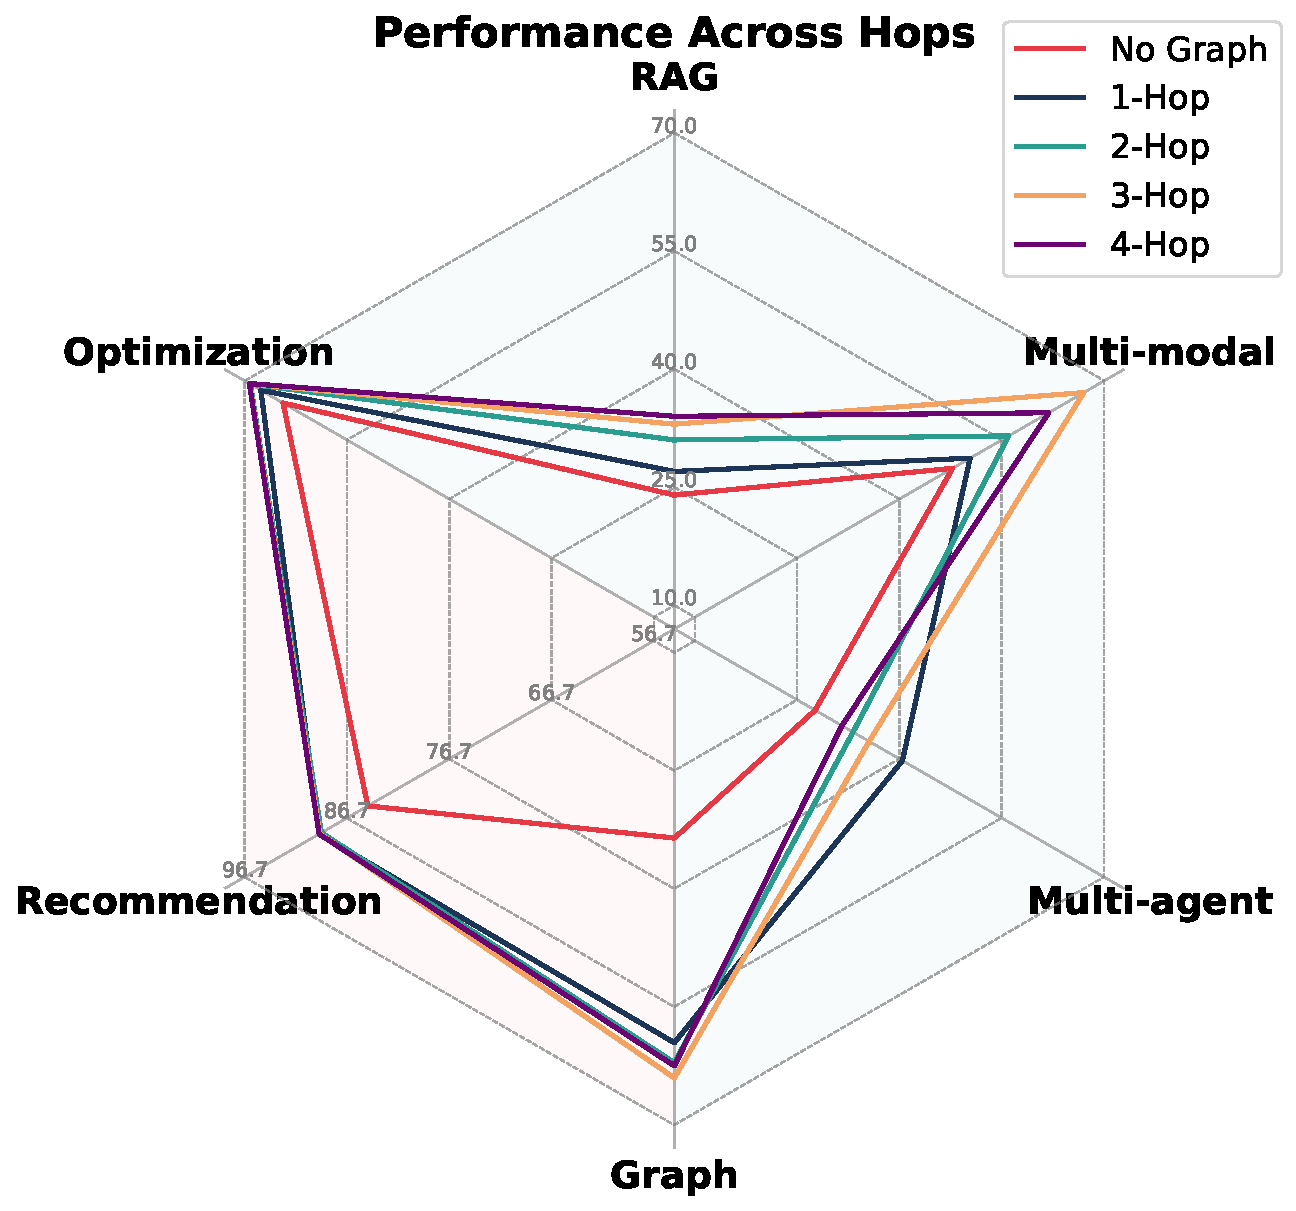
\includegraphics[width=\linewidth]{figs/hops_radar.pdf} 
\vspace{-4mm}
\caption{\textbf{Multi-hop graphs enhance GWM's performance across representative tasks in six domains}. We can observe that the introduction of graphs has benefited GWM-E across all tasks compared to no graph. Moreover, excessive hops can lead to over-smoothing, thereby decreasing performance.} %We can observe that the introduction of graphs has benefited GWM-E across all tasks compared to no graph. Moreover, excessive hops can lead to over-smoothing, thereby decreasing performance.
\label{fig:performance_hops}
\vspace{-3mm}
\end{figure}
% \begin{figure*}[ht]
% \centering
% \includegraphics[width=0.9\linewidth]{figs/performance_hops.pdf} 
% \vspace{-5mm}
% \caption{\textbf{Zero}.}
% \label{fig:performance_hops}
% \vspace{-3mm}
% \end{figure*}






% with graph/without graph/neighbourhood num
% different LLM backbones
% different LLM prompts
% different multi-modal encoders
% different graph models

\subsection{GWM boosts zero-shot/few-shot performance}

To validate the zero-shot/few-shot capabilities of GWM, we conduct experiments with GWM-E and GWM-T on the Agent and RAG tasks, as shown in Figure \ref{fig:zero_few_shot}  (``-T'' and ``-E'' respectively represent the experimental results of GWM-T and GWM-E). Here, Single Data refers to training GWM solely on the Agent or RAG task. Zero-shot refers to training GWM on tasks other than Agent or RAG and testing it on Agent or RAG. Fine-tuned GWM refers to training GWM on tasks other than Agent or RAG, followed by few-shot fine-tuning with 10\% of the data from Agent or RAG. We can observe that GWM adapts effectively to new tasks using only a small amount of domain-specific training data. Moreover, we observe that the zero-shot results of GWM on the RAG task are even better than those from Single Data, indicating that GWM's strong generalization ability greatly benefits tasks with limited training data like Agent or RAG.

%\vspace{-4mm}


% % zero-shots/few=shots/ learn from scratch


%% generalize across different domains:jointly learned 





% \begin{table}[h]
% \vspace{-0.1in}
% \caption{Zero-shot and few-shots.}
% \label{tab:zero}
% \vspace{-0.1in}
% \begin{center}
% \begin{small}
% \resizebox{1.05\columnwidth}{!}{
% \begin{sc}
% % \begin{tabular}{m{2.2cm}<{\centering}m{1.5cm}<{\centering}m{1.5cm}<{\centering}m{1cm}<{\centering}}
% \begin{tabular}{ccc}
% \toprule
% Train $\rightarrow$ Test  & Model & F1/Accuracy\\
% \midrule
% \multirow{3}*{\shortstack{All other \\ $\downarrow$ \\ Multi-agent collaboration}} 
% ~  & no GWM & 26.67  \\ %% no GWM
% ~  & Zero-shot & 10.67  \\
% ~  & Finetuned GWM & 35.56  \\ %% finetune GWM

% \midrule
% \multirow{3}*{\shortstack{All other \\ $\downarrow$ \\ Retrieval-augmented generation}} 
% ~  & no GWM & 25.49  \\
% ~  & Zero-shot & 24.57  \\
% ~  & Finetuned GWM & 33.32  \\
% \bottomrule
% \end{tabular}
% \end{sc}
% }
% \end{small}
% \end{center}
% \vskip -0.2in
% \end{table}


